 \chapter{Clustering}

%%%%%%%%%%%%%%%%%%%%%%%%%%%%%%%%%%%%%%%%%%%%%%%%%%%%%%%%%%%%%%%%%%%%%%%%%%%%%%%%%%%%%%%%%%
\section{K-means}
\subsection{Choice of attributes and distance function}

We have selected only $9$ of to performe the clustering via the K-Means algorithm.
In particular we have ignored the categorical attributes as there isn't a proper metric to define a distance function over these kinds of attributes.

So the used attributes are only: \textit{age}, \textit{limit}, \textit{ba\_mean}, \textit{pa-apr}, \textit{pa-may}, \textit{pa-jun}, \textit{pa-jul}, \textit{pa-aug}, \textit{pa-sep}.

For these attributes we uses the euclidean distance as the metric function.

\subsection{Choise of the best value of k}

To choose the best value of $k$ we have plotted for each $K$ between $2$ and $50$ the values of the SSE and the silhouette score. Each value is calculated as the best among $10$ runs (with the lowest SSE) and with a maximum of $300$ iterations of the K-Means algorithm.

\begin{figure}[h]
  \begin{minipage}[h]{.50\textwidth}
    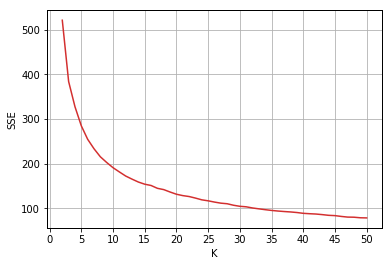
\includegraphics[width=1\textwidth]{img/ch3/kmeans_sse}
  \end{minipage}
    \begin{minipage}[h]{.50\textwidth}
    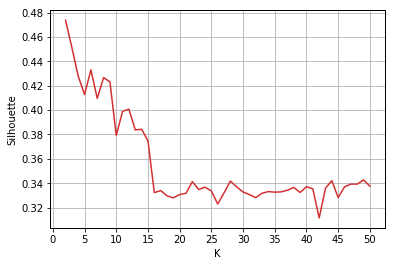
\includegraphics[width=1\textwidth]{img/ch3/kmeans_silhouette}
  \end{minipage}
\end{figure}

Using the elbow method we decide to set $k=5$ as it represents a good trade-off between SSE and data interpretability.

\subsection{Cluster analysis}

to do todo

%%%%%%%%%%%%%%%%%%%%%%%%%%%%%%%%%%%%%%%%%%%%%%%%%%%%%%%%%%%%%%%%%%%%%%%%%%%%%%%%%%%%%%%%%%
\section{DBSCAN}
\subsection{Choice of attributes and distance function}
\subsection{Study of the clustering parameters}
\subsection{Characterization and interpretation of the obtained clusters}
%%%%%%%%%%%%%%%%%%%%%%%%%%%%%%%%%%%%%%%%%%%%%%%%%%%%%%%%%%%%%%%%%%%%%%%%%%%%%%%%%%%%%%%%%%
\section{Hierarchical clustering}
\subsection{Choice of attributes and distance function}
\subsection{Discussion of dendograms using different algorithms}
%%%%%%%%%%%%%%%%%%%%%%%%%%%%%%%%%%%%%%%%%%%%%%%%%%%%%%%%%%%%%%%%%%%%%%%%%%%%%%%%%%%%%%%%%%

\section{Evaluation of clustering approaches and comparison of the clustering obtained}
